\subsection*{Textures} \label{sec:textures}
OpenGL does offer a way to draw images.
To draw an image you have to create a texture.
This texture is then passed to a shader.
You also have to create a VAO which contains vertices for a rectangle.
Each vertex has a position and a texture coordinate.
These texture coordinates are used to sample the texture using built-in shader functions.

Each image we want to draw can be represented by a texture.
For each image we want to draw, we can create a texture and pass it to the shader.
While this approach works, it is not very efficient.
Passing textures to the shader is a slow operation.
Because of that, we want to use as few textures as possible.
We can do that by combining multiple images into one.
We create Sprite Sheets which contain multiple images.
Each image in a sprite sheet (sprite) has a position and a size.
We can use this information to calculate the texture coordinates for each sprite.
We pass this information to the shader and use it to sample the correct part of the texture.
This way, we can pass a single texture to the shader and draw multiple images with it.

In our application, we have 2 sprite sheets.
The first one contains the images for the HUD.
This includes the inventory and all the items in it.
This sprite sheet is stored as a PNG file.
Sprite sheet with the inventory can be seen in \autoref*{fig:inventory}.
It also has a JSON file which contains the position and size of each sprite which can be seen in \autoref*{lst:inventory_sprite_sheet_json}.
The second sprite sheet contains the images of all letters and symbols used in the game.
This one is not stored in a file.
Instead, it is generated at runtime right after the program launches.
It uses SkiaSharp library to create a bitmap with all the ASCII characters.
This bitmap is then converted to a texture.
The position and size of each symbol is calculated using the font metrics.

These techniques are used to draw the HUD and the Menu.
Both of those are described in this chapter.

\begin{figure}[H]
    \centering
    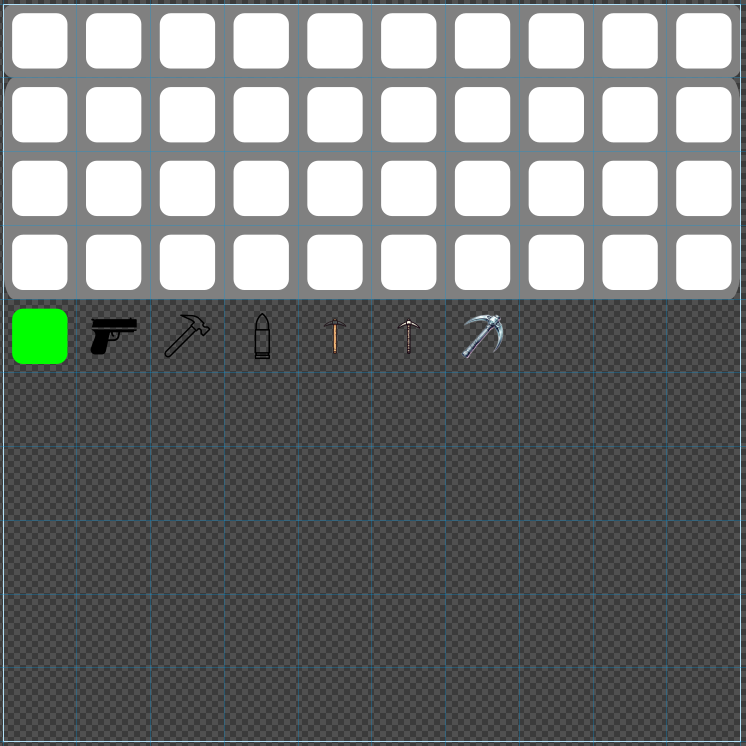
\includegraphics[width=0.8\textwidth]{chapters/two_dimensional_graphics/resources/SpriteSheet.png}
    \caption{Inventory Sprite Sheet}
    \label{fig:inventory}
\end{figure}
    
\begin{figure}[H]
    \begin{lstlisting}[language=json,firstline=1]
    {
        "width": 10,
        "height": 10,
        "items": [
            {
            "name": "hotbar",
            "x": 0,
            "y": 0,
            "width": 10,
            "height": 1
            },
        ]
    }
    \end{lstlisting}

    \caption{Inventory Sprite Sheet JSON}
    \label{lst:inventory_sprite_sheet_json}
\end{figure}